
 %%%%%%% SOFTWARE STRUCTURE %%%%%%
%\addcontentsline{toc}{section}{Software structure}
\section{Software structure}
\label{software_structure}

%In this section, the code functionalities of each part or node of the software are explained. The communication between nodes is shown and the overall software flow is thoroughly described. 

The code is structured in nodes. Each node contains a piece of the processing needed in the code. All nodes are related between them using ROS messages to transport the input and output data. 
\\

Computer vision is a field that involves high time-expensive algorithms. In the previous chapter it was explained that it uses 2D and 3D information. That information implies a matrix that has for each point 2 coordinates number (in the case of 2D) or 3 coordinates (in the case of 3D data), apart from the colour of that point, which is described using 3 more integers. \\

As it can be seen the data handled is enormous an the way to reduce the time lag due to those computations is modularizing the computation and executing in parallel those processes. 
\\

The software was designed to be as modular as was possible so that each node performs an action that could be used in other applications. 
As an example, the code could be easily changed to recognize hats or shoes, just changing the initial node that extracts the information of the desired joint. 
\\

In the following paragraphs the nodes' functionalities will be described and the communication between them presented. But first, the overall software work-flow is shown using the flow diagram below. 

\newpage
 %%%%%%% SOFTWARE FLOWCHART %%%%%%

\section{Software flowchart}

The input of the system is the information coming from the RGB-D sensor. There are two different data that are taken: the 2D information, i.e. the raw image detected by the sensor's camera, and the 3D information, i.e. the raw point cloud. Also, there is another input to the system that shows the position of the different user's joints. This data is provided by a third-party package called pi\_tracker that is explained in the following chapters. 
\\

The software was designed to be running on a robot as was previously explained. This implies that there can not be a GUI (G User Interface) on a screen because the robot being used might not have it. Also, the usability and easiness to learn how to interact with the program was important to allow different people not only investigators to use it. 
\\

In order to fulfil those requirements a gestural interface was designed. It is developed by a separate node so the processing lags will not affect the recognition of the different gestures. This fact also allows an easy change of the gestures being used. 
\\

The recognition of the location of the hand with respect to the user's body shows how the arm is positioned. If it is stretched towards the sensor, the software enters the dataset construction mode, i.e. the data acquisition and learning mode. If, otherwise, it is located closer to the body, the software starts the object recognition mode. 
\\

\begin{figure}[h]
	\begin{center}
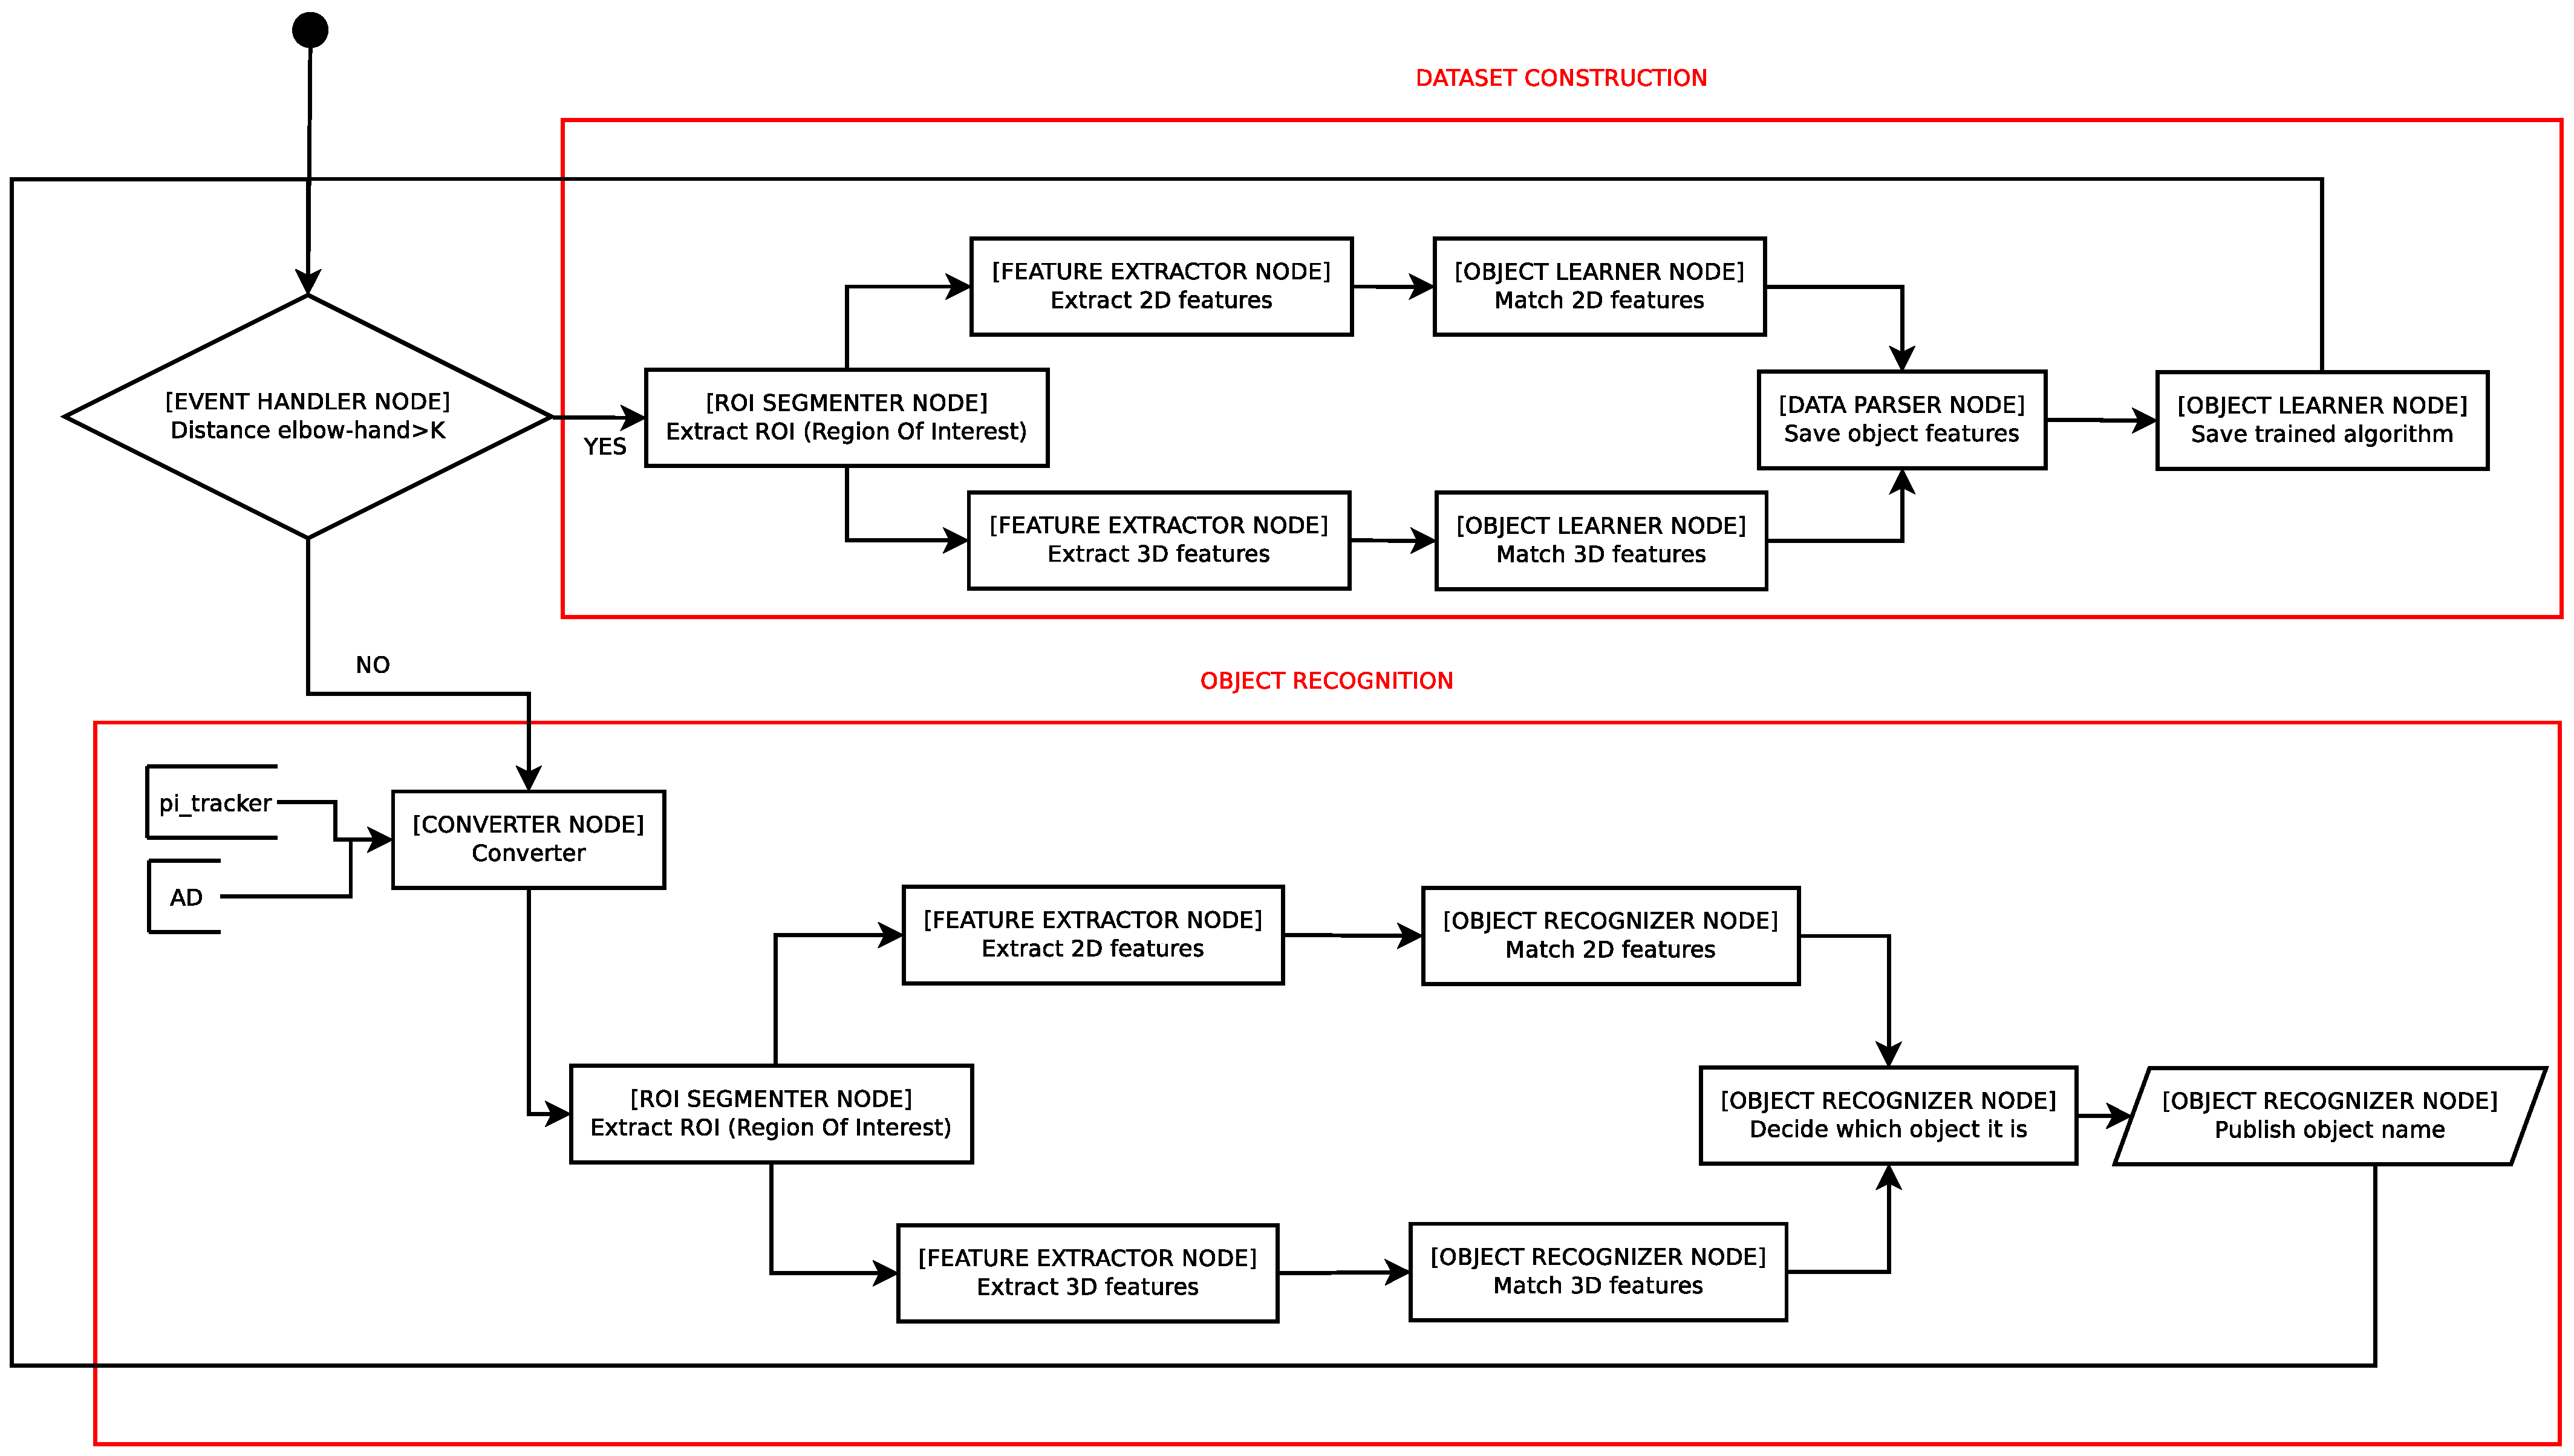
\includegraphics[scale=0.2]{img/diagrams/flowcharts.eps}
	\caption[Software flowchart]{Complete Software flowchart showing the different processing steps between the input and the output}
	\end{center}
\end{figure}


The upper part of the diagram shows the data acquisition work-flow. The first step is to extract the ROI (Region of Interest) from the input raw data. This is a crucial step that allows to reduce noticeably the amount of time due to computation reducing the size of the processed information. 
\\

After the extraction, the 2D and 3D features of the segmented data are obtained. The features or descriptors are characteristics that define and represent the data from where they were created. There are different algorithms that perform this task with better or worse repeatability and robustness. All the details about this process is explained in the next chapters. 
\\

That is the end of the data cycle of the learning process. It is iterated over the number of views for each object that is required in order to obtain all the templates necessary per object. 
\\

The recognition mode was triggered when the hand was located near the user's body. This mode can be seen in the lower part of the previous diagram. 
\\

The steps that compose this part of the software are the following: 
First, the input information is converted to the custom message used within the code. Afterwards, as in the previous mode, the Region Of Interest is segmented from both 2D and 3D original information. Then, the descriptors are extracted exactly the same way as in the previous mode. 
\\

The next step is the recognition algorithm. This matches the descriptors from both the image and the point cloud and decides which object of the dataset is more similar to the one that is currently on the user's hand. More details about this algorithm may be found in this section. 
\\

Finally, the object identification number is obtained. This data is the output of the system. 
